\documentclass[10pt,a4paper]{jsarticle}
\usepackage{listings,jlisting}
\usepackage{fancyhdr}
\usepackage{lastpage}
\usepackage[dvipdfmx]{graphicx,color}

\lhead{プログラミング実習IIレポート(第7回)}
\rhead{学籍番号:201811433 氏名:西田 直人}
\cfoot{\thepage/\pageref{LastPage}}

\pagestyle{fancy}

\title{プログラミングII実習レポート課題第7回}
\author{西田直人}

\begin{document}
%\markright{プログラミング実習1Aレポート(第1回) 学籍番号:201811433 氏名:西田直人}
%\maketitle
\begin{center}
{\LARGE プログラミング実習IIレポート課題第7回} \\
\large
西田直人 \\ 2019年1月18日
\end{center}
\normalsize
\section{課題7-1}
\subsection{誤っている箇所}

\subsection{source}
\lstinputlisting[basicstyle=\ttfamily\footnotesize,frame=single,breaklines=tr\
ue,caption=a1-1.c]{a1-1.c}

\subsection{result}

\begin{lstlisting}[basicstyle=\ttfamily\footnotesize,frame=single,breaklines=tr\
  ue,caption=]
     
\end{lstlisting}


\section{課題1-2}

\subsection{source}
\lstinputlisting[basicstyle=\ttfamily\footnotesize,frame=single,breaklines=tr\
  ue,caption=a1-1.c]{a1-1.c}


\subsection{result}
\begin{lstlisting}[basicstyle=\ttfamily\footnotesize,frame=single,breaklines=tr\
  ue,caption=]
  
\end{lstlisting}

\section{課題1-3}
\subsection{source}
\lstinputlisting[basicstyle=\ttfamily\footnotesize,frame=single,breaklines=tr\
ue,caption=]{a1-3.c}

\subsection{result}

\begin{lstlisting}[basicstyle=\ttfamily\footnotesize,frame=single,breaklines=tr\
  ue,caption=]
  
\end{lstlisting}

\begin{figure}[h]
  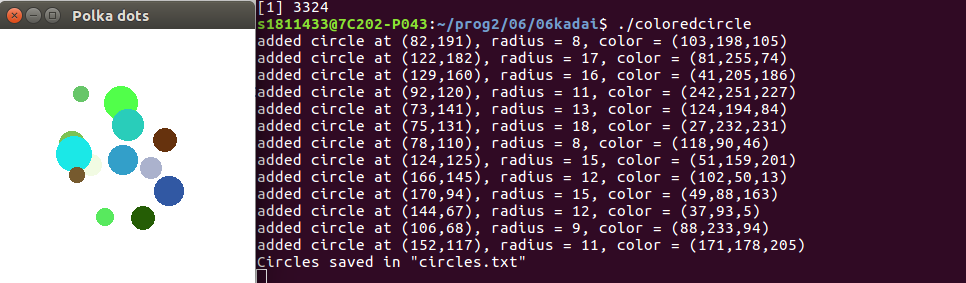
\includegraphics[width=0.8\linewidth]{b.png}
  \caption{数回クリックしたあとにsを押した}
  \label{fig:sutehage}
  

\end{document}
